% Created by tikzDevice version 0.6.2-92-0ad2792 on 2013-11-12 08:12:24
% !TEX encoding = UTF-8 Unicode
\documentclass[12pt, mainfont = Minion,     mainscale = 1.0, sansfont = Myriad,     sansscale = MatchLowercase, monofont = Consolas,   monoscale = MatchLowercase, mathfont = MinionMath, mathscale = 1.0]{mtikzfig}
\begin{document}

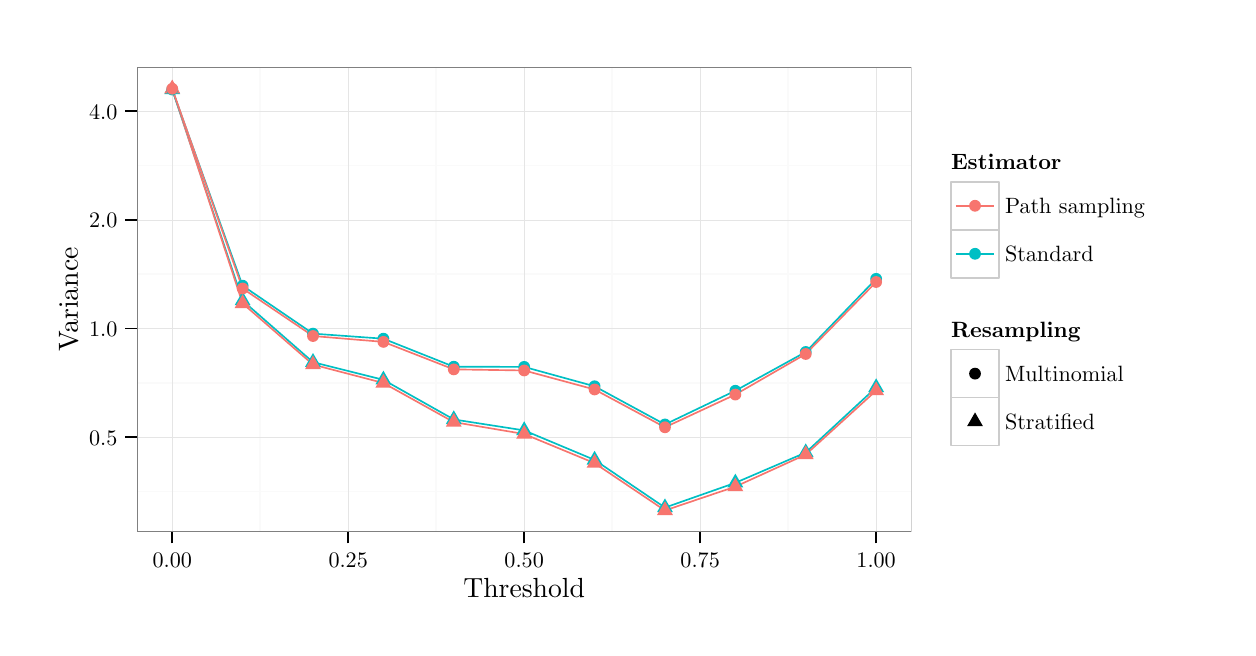
\begin{tikzpicture}[x=1pt,y=1pt]
\definecolor[named]{fillColor}{rgb}{1.00,1.00,1.00}
\path[use as bounding box,fill=fillColor,fill opacity=0.00] (0,0) rectangle (433.62,216.81);
\begin{scope}
\path[clip] (  0.00,  0.00) rectangle (433.62,216.81);
\definecolor[named]{drawColor}{rgb}{1.00,1.00,1.00}
\definecolor[named]{fillColor}{rgb}{1.00,1.00,1.00}

\path[draw=drawColor,line width= 0.6pt,line join=round,line cap=round,fill=fillColor] (  0.00,  0.00) rectangle (433.62,216.81);
\end{scope}
\begin{scope}
\path[clip] ( 39.51, 34.74) rectangle (319.31,202.36);
\definecolor[named]{fillColor}{rgb}{1.00,1.00,1.00}

\path[fill=fillColor] ( 39.51, 34.74) rectangle (319.31,202.36);
\definecolor[named]{drawColor}{rgb}{0.98,0.98,0.98}

\path[draw=drawColor,line width= 0.6pt,line join=round] ( 39.51, 49.25) --
	(319.31, 49.25);

\path[draw=drawColor,line width= 0.6pt,line join=round] ( 39.51, 88.49) --
	(319.31, 88.49);

\path[draw=drawColor,line width= 0.6pt,line join=round] ( 39.51,127.74) --
	(319.31,127.74);

\path[draw=drawColor,line width= 0.6pt,line join=round] ( 39.51,166.99) --
	(319.31,166.99);

\path[draw=drawColor,line width= 0.6pt,line join=round] ( 84.02, 34.74) --
	( 84.02,202.36);

\path[draw=drawColor,line width= 0.6pt,line join=round] (147.61, 34.74) --
	(147.61,202.36);

\path[draw=drawColor,line width= 0.6pt,line join=round] (211.20, 34.74) --
	(211.20,202.36);

\path[draw=drawColor,line width= 0.6pt,line join=round] (274.79, 34.74) --
	(274.79,202.36);
\definecolor[named]{drawColor}{rgb}{0.90,0.90,0.90}

\path[draw=drawColor,line width= 0.2pt,line join=round] ( 39.51, 68.87) --
	(319.31, 68.87);

\path[draw=drawColor,line width= 0.2pt,line join=round] ( 39.51,108.12) --
	(319.31,108.12);

\path[draw=drawColor,line width= 0.2pt,line join=round] ( 39.51,147.37) --
	(319.31,147.37);

\path[draw=drawColor,line width= 0.2pt,line join=round] ( 39.51,186.61) --
	(319.31,186.61);

\path[draw=drawColor,line width= 0.2pt,line join=round] ( 52.23, 34.74) --
	( 52.23,202.36);

\path[draw=drawColor,line width= 0.2pt,line join=round] (115.82, 34.74) --
	(115.82,202.36);

\path[draw=drawColor,line width= 0.2pt,line join=round] (179.41, 34.74) --
	(179.41,202.36);

\path[draw=drawColor,line width= 0.2pt,line join=round] (243.00, 34.74) --
	(243.00,202.36);

\path[draw=drawColor,line width= 0.2pt,line join=round] (306.59, 34.74) --
	(306.59,202.36);
\definecolor[named]{drawColor}{rgb}{0.00,0.75,0.77}

\path[draw=drawColor,line width= 0.6pt,line join=round] ( 52.23,194.46) --
	( 77.67,118.17) --
	(103.10, 95.93) --
	(128.54, 89.56) --
	(153.97, 75.24) --
	(179.41, 71.28) --
	(204.85, 60.62) --
	(230.28, 43.39) --
	(255.72, 52.34) --
	(281.15, 63.28) --
	(306.59, 86.81);
\definecolor[named]{drawColor}{rgb}{0.97,0.46,0.43}

\path[draw=drawColor,line width= 0.6pt,line join=round] ( 52.23,194.74) --
	( 77.67,117.16) --
	(103.10, 95.06) --
	(128.54, 88.41) --
	(153.97, 74.28) --
	(179.41, 69.98) --
	(204.85, 59.46) --
	(230.28, 42.36) --
	(255.72, 50.96) --
	(281.15, 62.55) --
	(306.59, 85.66);
\definecolor[named]{drawColor}{rgb}{0.00,0.75,0.77}

\path[draw=drawColor,line width= 0.6pt,line join=round] ( 52.23,194.46) --
	( 77.67,123.57) --
	(103.10,106.25) --
	(128.54,104.42) --
	(153.97, 94.30) --
	(179.41, 94.23) --
	(204.85, 87.23) --
	(230.28, 73.43) --
	(255.72, 85.62) --
	(281.15, 99.62) --
	(306.59,126.05);
\definecolor[named]{drawColor}{rgb}{0.97,0.46,0.43}

\path[draw=drawColor,line width= 0.6pt,line join=round] ( 52.23,194.74) --
	( 77.67,122.56) --
	(103.10,105.38) --
	(128.54,103.27) --
	(153.97, 93.33) --
	(179.41, 92.94) --
	(204.85, 86.07) --
	(230.28, 72.41) --
	(255.72, 84.24) --
	(281.15, 98.90) --
	(306.59,124.91);
\definecolor[named]{fillColor}{rgb}{0.00,0.75,0.77}

\path[fill=fillColor] ( 52.23,197.78) --
	( 55.10,192.80) --
	( 49.36,192.80) --
	cycle;

\path[fill=fillColor] ( 77.67,121.49) --
	( 80.54,116.52) --
	( 74.79,116.52) --
	cycle;

\path[fill=fillColor] (103.10, 99.25) --
	(105.98, 94.27) --
	(100.23, 94.27) --
	cycle;

\path[fill=fillColor] (128.54, 92.88) --
	(131.41, 87.90) --
	(125.66, 87.90) --
	cycle;

\path[fill=fillColor] (153.97, 78.56) --
	(156.85, 73.58) --
	(151.10, 73.58) --
	cycle;

\path[fill=fillColor] (179.41, 74.59) --
	(182.28, 69.62) --
	(176.54, 69.62) --
	cycle;

\path[fill=fillColor] (204.85, 63.93) --
	(207.72, 58.96) --
	(201.97, 58.96) --
	cycle;

\path[fill=fillColor] (230.28, 46.71) --
	(233.16, 41.73) --
	(227.41, 41.73) --
	cycle;

\path[fill=fillColor] (255.72, 55.66) --
	(258.59, 50.68) --
	(252.84, 50.68) --
	cycle;

\path[fill=fillColor] (281.15, 66.59) --
	(284.03, 61.62) --
	(278.28, 61.62) --
	cycle;

\path[fill=fillColor] (306.59, 90.12) --
	(309.46, 85.15) --
	(303.72, 85.15) --
	cycle;
\definecolor[named]{fillColor}{rgb}{0.97,0.46,0.43}

\path[fill=fillColor] ( 52.23,198.06) --
	( 55.10,193.08) --
	( 49.36,193.08) --
	cycle;

\path[fill=fillColor] ( 77.67,120.48) --
	( 80.54,115.50) --
	( 74.79,115.50) --
	cycle;

\path[fill=fillColor] (103.10, 98.38) --
	(105.98, 93.40) --
	(100.23, 93.40) --
	cycle;

\path[fill=fillColor] (128.54, 91.73) --
	(131.41, 86.75) --
	(125.66, 86.75) --
	cycle;

\path[fill=fillColor] (153.97, 77.60) --
	(156.85, 72.62) --
	(151.10, 72.62) --
	cycle;

\path[fill=fillColor] (179.41, 73.30) --
	(182.28, 68.32) --
	(176.54, 68.32) --
	cycle;

\path[fill=fillColor] (204.85, 62.78) --
	(207.72, 57.80) --
	(201.97, 57.80) --
	cycle;

\path[fill=fillColor] (230.28, 45.68) --
	(233.16, 40.70) --
	(227.41, 40.70) --
	cycle;

\path[fill=fillColor] (255.72, 54.27) --
	(258.59, 49.30) --
	(252.84, 49.30) --
	cycle;

\path[fill=fillColor] (281.15, 65.87) --
	(284.03, 60.89) --
	(278.28, 60.89) --
	cycle;

\path[fill=fillColor] (306.59, 88.98) --
	(309.46, 84.00) --
	(303.72, 84.00) --
	cycle;
\definecolor[named]{fillColor}{rgb}{0.00,0.75,0.77}

\path[fill=fillColor] ( 52.23,194.46) circle (  2.13);

\path[fill=fillColor] ( 77.67,123.57) circle (  2.13);

\path[fill=fillColor] (103.10,106.25) circle (  2.13);

\path[fill=fillColor] (128.54,104.42) circle (  2.13);

\path[fill=fillColor] (153.97, 94.30) circle (  2.13);

\path[fill=fillColor] (179.41, 94.23) circle (  2.13);

\path[fill=fillColor] (204.85, 87.23) circle (  2.13);

\path[fill=fillColor] (230.28, 73.43) circle (  2.13);

\path[fill=fillColor] (255.72, 85.62) circle (  2.13);

\path[fill=fillColor] (281.15, 99.62) circle (  2.13);

\path[fill=fillColor] (306.59,126.05) circle (  2.13);
\definecolor[named]{fillColor}{rgb}{0.97,0.46,0.43}

\path[fill=fillColor] ( 52.23,194.74) circle (  2.13);

\path[fill=fillColor] ( 77.67,122.56) circle (  2.13);

\path[fill=fillColor] (103.10,105.38) circle (  2.13);

\path[fill=fillColor] (128.54,103.27) circle (  2.13);

\path[fill=fillColor] (153.97, 93.33) circle (  2.13);

\path[fill=fillColor] (179.41, 92.94) circle (  2.13);

\path[fill=fillColor] (204.85, 86.07) circle (  2.13);

\path[fill=fillColor] (230.28, 72.41) circle (  2.13);

\path[fill=fillColor] (255.72, 84.24) circle (  2.13);

\path[fill=fillColor] (281.15, 98.90) circle (  2.13);

\path[fill=fillColor] (306.59,124.91) circle (  2.13);
\definecolor[named]{drawColor}{rgb}{0.50,0.50,0.50}

\path[draw=drawColor,line width= 0.6pt,line join=round,line cap=round] ( 39.51, 34.74) rectangle (319.31,202.36);
\end{scope}
\begin{scope}
\path[clip] (  0.00,  0.00) rectangle (433.62,216.81);
\definecolor[named]{drawColor}{rgb}{0.00,0.00,0.00}

\node[text=drawColor,anchor=base east,inner sep=0pt, outer sep=0pt, scale=  0.80] at ( 32.40, 65.94) {0.5};

\node[text=drawColor,anchor=base east,inner sep=0pt, outer sep=0pt, scale=  0.80] at ( 32.40,105.19) {1.0};

\node[text=drawColor,anchor=base east,inner sep=0pt, outer sep=0pt, scale=  0.80] at ( 32.40,144.44) {2.0};

\node[text=drawColor,anchor=base east,inner sep=0pt, outer sep=0pt, scale=  0.80] at ( 32.40,183.69) {4.0};
\end{scope}
\begin{scope}
\path[clip] (  0.00,  0.00) rectangle (433.62,216.81);
\definecolor[named]{drawColor}{rgb}{0.00,0.00,0.00}

\path[draw=drawColor,line width= 0.6pt,line join=round] ( 35.24, 68.87) --
	( 39.51, 68.87);

\path[draw=drawColor,line width= 0.6pt,line join=round] ( 35.24,108.12) --
	( 39.51,108.12);

\path[draw=drawColor,line width= 0.6pt,line join=round] ( 35.24,147.37) --
	( 39.51,147.37);

\path[draw=drawColor,line width= 0.6pt,line join=round] ( 35.24,186.61) --
	( 39.51,186.61);
\end{scope}
\begin{scope}
\path[clip] (  0.00,  0.00) rectangle (433.62,216.81);
\definecolor[named]{drawColor}{rgb}{0.00,0.00,0.00}

\path[draw=drawColor,line width= 0.6pt,line join=round] ( 52.23, 30.47) --
	( 52.23, 34.74);

\path[draw=drawColor,line width= 0.6pt,line join=round] (115.82, 30.47) --
	(115.82, 34.74);

\path[draw=drawColor,line width= 0.6pt,line join=round] (179.41, 30.47) --
	(179.41, 34.74);

\path[draw=drawColor,line width= 0.6pt,line join=round] (243.00, 30.47) --
	(243.00, 34.74);

\path[draw=drawColor,line width= 0.6pt,line join=round] (306.59, 30.47) --
	(306.59, 34.74);
\end{scope}
\begin{scope}
\path[clip] (  0.00,  0.00) rectangle (433.62,216.81);
\definecolor[named]{drawColor}{rgb}{0.00,0.00,0.00}

\node[text=drawColor,anchor=base,inner sep=0pt, outer sep=0pt, scale=  0.80] at ( 52.23, 21.77) {0.00};

\node[text=drawColor,anchor=base,inner sep=0pt, outer sep=0pt, scale=  0.80] at (115.82, 21.77) {0.25};

\node[text=drawColor,anchor=base,inner sep=0pt, outer sep=0pt, scale=  0.80] at (179.41, 21.77) {0.50};

\node[text=drawColor,anchor=base,inner sep=0pt, outer sep=0pt, scale=  0.80] at (243.00, 21.77) {0.75};

\node[text=drawColor,anchor=base,inner sep=0pt, outer sep=0pt, scale=  0.80] at (306.59, 21.77) {1.00};
\end{scope}
\begin{scope}
\path[clip] (  0.00,  0.00) rectangle (433.62,216.81);
\definecolor[named]{drawColor}{rgb}{0.00,0.00,0.00}

\node[text=drawColor,anchor=base,inner sep=0pt, outer sep=0pt, scale=  1.00] at (179.41, 10.84) {Threshold};
\end{scope}
\begin{scope}
\path[clip] (  0.00,  0.00) rectangle (433.62,216.81);
\definecolor[named]{drawColor}{rgb}{0.00,0.00,0.00}

\node[text=drawColor,rotate= 90.00,anchor=base,inner sep=0pt, outer sep=0pt, scale=  1.00] at ( 18.16,118.55) {Variance};
\end{scope}
\begin{scope}
\path[clip] (  0.00,  0.00) rectangle (433.62,216.81);
\definecolor[named]{fillColor}{rgb}{1.00,1.00,1.00}

\path[fill=fillColor] (329.38,122.16) rectangle (409.09,175.58);
\end{scope}
\begin{scope}
\path[clip] (  0.00,  0.00) rectangle (433.62,216.81);
\definecolor[named]{drawColor}{rgb}{0.00,0.00,0.00}

\node[text=drawColor,anchor=base west,inner sep=0pt, outer sep=0pt, scale=  0.80] at (333.65,165.46) {\bfseries Estimator};
\end{scope}
\begin{scope}
\path[clip] (  0.00,  0.00) rectangle (433.62,216.81);
\definecolor[named]{drawColor}{rgb}{0.80,0.80,0.80}
\definecolor[named]{fillColor}{rgb}{1.00,1.00,1.00}

\path[draw=drawColor,line width= 0.6pt,line join=round,line cap=round,fill=fillColor] (333.65,143.78) rectangle (350.99,161.12);
\end{scope}
\begin{scope}
\path[clip] (  0.00,  0.00) rectangle (433.62,216.81);
\definecolor[named]{drawColor}{rgb}{0.97,0.46,0.43}

\path[draw=drawColor,line width= 0.6pt,line join=round] (335.38,152.45) -- (349.26,152.45);
\end{scope}
\begin{scope}
\path[clip] (  0.00,  0.00) rectangle (433.62,216.81);
\definecolor[named]{fillColor}{rgb}{0.97,0.46,0.43}

\path[fill=fillColor] (342.32,152.45) circle (  2.13);
\end{scope}
\begin{scope}
\path[clip] (  0.00,  0.00) rectangle (433.62,216.81);
\definecolor[named]{drawColor}{rgb}{0.80,0.80,0.80}
\definecolor[named]{fillColor}{rgb}{1.00,1.00,1.00}

\path[draw=drawColor,line width= 0.6pt,line join=round,line cap=round,fill=fillColor] (333.65,126.43) rectangle (350.99,143.78);
\end{scope}
\begin{scope}
\path[clip] (  0.00,  0.00) rectangle (433.62,216.81);
\definecolor[named]{drawColor}{rgb}{0.00,0.75,0.77}

\path[draw=drawColor,line width= 0.6pt,line join=round] (335.38,135.10) -- (349.26,135.10);
\end{scope}
\begin{scope}
\path[clip] (  0.00,  0.00) rectangle (433.62,216.81);
\definecolor[named]{fillColor}{rgb}{0.00,0.75,0.77}

\path[fill=fillColor] (342.32,135.10) circle (  2.13);
\end{scope}
\begin{scope}
\path[clip] (  0.00,  0.00) rectangle (433.62,216.81);
\definecolor[named]{drawColor}{rgb}{0.00,0.00,0.00}

\node[text=drawColor,anchor=base west,inner sep=0pt, outer sep=0pt, scale=  0.80] at (353.16,149.52) {Path sampling};
\end{scope}
\begin{scope}
\path[clip] (  0.00,  0.00) rectangle (433.62,216.81);
\definecolor[named]{drawColor}{rgb}{0.00,0.00,0.00}

\node[text=drawColor,anchor=base west,inner sep=0pt, outer sep=0pt, scale=  0.80] at (353.16,132.18) {Standard};
\end{scope}
\begin{scope}
\path[clip] (  0.00,  0.00) rectangle (433.62,216.81);
\definecolor[named]{fillColor}{rgb}{1.00,1.00,1.00}

\path[fill=fillColor] (329.38, 61.52) rectangle (401.29,114.94);
\end{scope}
\begin{scope}
\path[clip] (  0.00,  0.00) rectangle (433.62,216.81);
\definecolor[named]{drawColor}{rgb}{0.00,0.00,0.00}

\node[text=drawColor,anchor=base west,inner sep=0pt, outer sep=0pt, scale=  0.80] at (333.65,104.81) {\bfseries Resampling};
\end{scope}
\begin{scope}
\path[clip] (  0.00,  0.00) rectangle (433.62,216.81);
\definecolor[named]{drawColor}{rgb}{0.80,0.80,0.80}
\definecolor[named]{fillColor}{rgb}{1.00,1.00,1.00}

\path[draw=drawColor,line width= 0.6pt,line join=round,line cap=round,fill=fillColor] (333.65, 83.13) rectangle (350.99,100.48);
\end{scope}
\begin{scope}
\path[clip] (  0.00,  0.00) rectangle (433.62,216.81);
\definecolor[named]{fillColor}{rgb}{0.00,0.00,0.00}

\path[fill=fillColor] (342.32, 91.80) circle (  2.13);
\end{scope}
\begin{scope}
\path[clip] (  0.00,  0.00) rectangle (433.62,216.81);
\definecolor[named]{drawColor}{rgb}{0.80,0.80,0.80}
\definecolor[named]{fillColor}{rgb}{1.00,1.00,1.00}

\path[draw=drawColor,line width= 0.6pt,line join=round,line cap=round,fill=fillColor] (333.65, 65.79) rectangle (350.99, 83.13);
\end{scope}
\begin{scope}
\path[clip] (  0.00,  0.00) rectangle (433.62,216.81);
\definecolor[named]{fillColor}{rgb}{0.00,0.00,0.00}

\path[fill=fillColor] (342.32, 77.78) --
	(345.19, 72.80) --
	(339.45, 72.80) --
	cycle;
\end{scope}
\begin{scope}
\path[clip] (  0.00,  0.00) rectangle (433.62,216.81);
\definecolor[named]{drawColor}{rgb}{0.00,0.00,0.00}

\node[text=drawColor,anchor=base west,inner sep=0pt, outer sep=0pt, scale=  0.80] at (353.16, 88.88) {Multinomial};
\end{scope}
\begin{scope}
\path[clip] (  0.00,  0.00) rectangle (433.62,216.81);
\definecolor[named]{drawColor}{rgb}{0.00,0.00,0.00}

\node[text=drawColor,anchor=base west,inner sep=0pt, outer sep=0pt, scale=  0.80] at (353.16, 71.53) {Stratified};
\end{scope}
\end{tikzpicture}

\end{document}
